\documentclass[12pt]{article}
\usepackage{amsmath,amssymb,amsfonts}
\usepackage{geometry}
\usepackage{hyperref}
\usepackage{graphicx}
\usepackage{tikz}
\usetikzlibrary{arrows.meta, positioning, shapes.geometric}
\usepackage{booktabs}
\usepackage{enumitem}
\geometry{letterpaper,margin=1in}

\title{Ethics-Constrained Economic Mechanisms on Tau Net:\\
The Alignment Theorem and the Virtuous Cycle Compounder}
\author{Tau Alignment Research Group\\
\small{\texttt{research@taunet.org}}}
\date{December 2025}

\begin{document}
\maketitle

\begin{abstract}
This paper formalizes the \emph{Alignment Theorem}, an economics-driven approach to ensuring that all rational agents operating on Tau Net converge toward ethical behavior. Tau's knowledge representation and preference aggregation stack enables the network to maintain a live consensus over ethical worldviews; this consensus is encoded in the Ethical-Eco Transaction Factor (EETF) signal that drives the economics of the Virtuous Cycle Compounder (VCC). We present (i) the ethics aggregation pipeline, (ii) a Lean~4 proof that enforces ethical optimality under scarcity-driven pressure, and (iii) the executable Tau specifications and visual analytics (VCC Concept Visualizer) that instantiate the theory. Together, these results demonstrate a fully verifiable architecture for ethics-aware, deflationary agents on the Tau blockchain.
\end{abstract}

\textbf{Keywords:} Tau Net, Alignment Theorem, ethical consensus, Lean proof, Virtuous Cycle Compounder, deflationary economics.

\section{Introduction}
Ensuring that autonomous economic agents behave ethically remains a central challenge for decentralized systems. Traditional approaches rely on static rule sets or exogenous governance, both of which fail to keep pace with adaptive, multi-agent environments. Tau Net offers a fundamentally different path: users describe their ethical preferences in a machine-readable logic, Tau aggregates those preferences into a global consensus (the EETF), and economic agents must optimize against that consensus to remain profitable. The Alignment Theorem gives the theoretical underpinning for this scheme by proving that, under scarcity-driven pressure and infinite token divisibility, ethical behavior becomes the only rational equilibrium.

We extend earlier drafts of the theorem with three key advances:
\begin{enumerate}[leftmargin=*]
    \item A formal ethics pipeline that maps knowledge-representation artifacts into the network-wide EETF signal.
    \item A Lean~4 mechanization of the theorem that eliminates prior ``\texttt{sorry}'' placeholders and explains the role of infinite divisibility.
    \item An academic-ready exposition linking the proof to the Virtuous Cycle Compounder (VCC) educational platform~\cite{vccviz}, which demonstrates the theorem's implications through interactive visualizations.
\end{enumerate}

\section{Background}
\subsection{Tau Language and Knowledge Representation}
Tau Language is an executable formal specification framework designed for program synthesis and verifiable smart contracts. Its pointwise revision semantics allow live specifications to consume community knowledge, while its underlying Binary Decision Diagram (BDD) optimizations keep formal verification tractable. Users encode ethical models as logical theories, which are then broadcast and aggregated through Tau's knowledge graph. When native reasoning modules become available, each account's ethical worldview will be both machine-checkable and auditable on-chain, enabling a continuously updated consensus signal.

\subsection{Ethics Aggregation and the EETF Signal}
Let $\mathcal{M}=\{m_i\}_{i=1}^N$ denote the set of ethical models published by users. Tau's aggregation operator $\mathcal{A}$ combines these models (via preference aggregation, proof-of-consensus voting, or knowledge-based arbitration) into a bounded real number $E(t)=\mathcal{A}(\mathcal{M},t) \in [0,3]$. This quantity acts as the network-wide Ethical-Eco Transaction Factor (EETF), which scales rewards and penalties in all alignment-aware agents. In practice, $\mathcal{A}$ is implemented through Tau Language specifications that track attestations, weights, and model validity proofs.

\subsection{Virtuous Cycle Compounder (VCC)}
The Virtuous Cycle Compounder integrates three mechanisms - Dynamic Base Reward (DBR), Hyper-Compounding Rewards (HCR), and Aggressive Ethical Burn (AEB) - to reinforce ethical behavior through deflationary economics. Importantly, AEB is \emph{not} a punishment track: higher collective ethics ($E(t)$ above threshold) unlocks bonus burns that permanently remove supply as a \emph{reward} for virtuous flows, increasing scarcity for all aligned holders. Its concept visualizer~\cite{vccviz} provides an interactive explanation, including TEEC foundations, mathematical tooltips, and evolution diagrams linking ethics to scarcity. VCC agents consume the EETF signal produced by the Alignment Theorem's pipeline, ensuring that the theorem is not merely theoretical but realized in executable Tau specifications.

\subsection{Verification and Visualization Stack}
Three layers keep the theory honest. First, a Lean~4 development discharges the Alignment Theorem without unproven axioms, so the scarcity threshold argument is mechanically checked. Second, Tau agents (v35--v54 plus shared libraries) execute both in the native interpreter and in an exact Python simulator, giving identical FSM traces for coverage and invariant testing. Third, stakeholder-facing dashboards - the Alignment Theorem single-page app and the VCC concept explorer - show how live changes in $E(t)$ ripple through DBR/HCR/AEB, making the incentive surface auditable for non-developers.

\subsection{Tau Testnet Substrate and Extralogical Primitives}
The tau-testnet reference implementation~\cite{tautestnet} treats Tau specifications as first-class chain data. Every revision transaction is replayed pointwise so only the targeted formulas change, and validation logic re-applies the Tau engine before admitting rule edits to the mempool. The runtime exposes an extralogical API for BLS verification, commit-reveal patterns, networking, and storage, giving DBR/HCR/AEB contracts a trustworthy way to call cryptography and IO from within Tau rules while keeping the logical kernel minimal. Preference aggregation rules can therefore encode utilitarian or ranked-choice logic directly in Tau: users post logical formulas describing utilities or priorities, optionally commit-and-reveal them for fairness, and the aggregation spec merges them into the consensus EETF signal.

\subsection{Preference-Utilitarian Aggregation}
Tau's declarative setup allows us to implement preference utilitarianism in the style of Harsanyi's additive social welfare functional~\cite{preferencebased}. Each agent exposes a logical preference relation or a utility function symbol $u_i$; axioms enforce transitivity, completeness, and affine comparability so that utilities can be summed. Commit-reveal flows protect the submission of utilities or ranked judgments, and aggregation specs can encode utilitarian sums, distance-based belief merging, or ranked-choice rules similar to those studied in logic-based social choice and machine ethics~\cite{machineethics,ca_utilitarian}. Because the aggregation contract is itself a Tau specification, every assumption (summing weights, normalizing utilities, handling missing data) remains auditable and formally verifiable.

\section{Formal Model}
\subsection{Normalized Supply and Scarcity}
Let $S(t)$ denote the normalized (real-valued) token supply at discrete time $t$ with initial value $S(0)=S_0>0$. We assume a bounded deflation rate $r(t)\in [0.01,0.50]$ such that:
\[
S(t+1) = S(t)\cdot \big(1-r(t)\big).
\]
While $S(t)\rightarrow 0$ asymptotically in $\mathbb{R}$, the on-chain AGRS token remains usable thanks to infinite divisibility (decimal shifting, analogous to Bitcoin sats). Scarcity is defined as $M(t)=S_0/S(t)$, which diverges to $+\infty$ as $t\rightarrow\infty$.

\subsection{Economic Pressure and Ethics}
Given the network EETF $E(t)>0$ the economic pressure is:
\[
P(t)=M(t)\cdot E(t).
\]
The consensus EETF acts as a live ``ethics oracle'', meaning that Tau's knowledge-driven aggregation determines $E(t)$ in real time. This is the point where preference aggregation and knowledge representation become crucial: if users update or redefine ethics, $E(t)$ updates accordingly without altering the Alignment Theorem's structure.

\subsection{Reward and Penalty Functions}
For any agent with balance $B>0$, transaction exposure $X>0$, and account-level EETF $e\in[0,3]$, the expected value is:
\[
\mathrm{EV}(e,t) = \frac{B\cdot M(t)\cdot \mathrm{tier}(e)}{1000} - \frac{X\cdot (1-e)\cdot P(t)}{100},
\]
where $\mathrm{tier}(e)$ is a piecewise constant multiplier (1, 3, or 5) for ethical tiers. Ethical agents ($e\ge 1$) receive strictly positive rewards and zero penalties, while unethical agents ($e<1$) obtain zero rewards and increasing penalties as $P(t)$ grows.

\section{Lean~4 Formalization}
\subsection{Definitions}
We encode the above structures in Lean~4 (file \texttt{proofs/AlignmentTheorem.lean}). The file defines:
\begin{itemize}[leftmargin=*]
    \item \texttt{Supply}, \texttt{EETF}, and \texttt{DeflationRate} structures with positivity and boundedness proofs.
    \item Functions \texttt{scarcity}, \texttt{economicPressure}, and \texttt{expectedValue}.
    \item Auxiliary lemmas such as \texttt{scarcity\_limit\_infinity}, which captures the divergence of $M(t)$.
\end{itemize}

\subsection{Core Lemmas}
\begin{enumerate}[leftmargin=*]
    \item \textbf{Ethical EV positivity:} \texttt{expectedValue\_baseline\_pos} shows that ethical agents always yield strictly positive EV once scarcity is positive.
    \item \textbf{Unethical EV negativity:} \texttt{expectedValue\_unethical\_neg} proves that any agent with $e<1$ faces negative EV as soon as it participates in the system.
    \item \textbf{Alignment theorem:} Given a rational choice function that maximizes EV over all available EETF states, the Lean proof concludes that the agent must eventually adopt $e\ge 1$.
\end{enumerate}

\subsection{Lean Tooling}
We built the proof using the standard Tau research toolchain with Mathlib, Aesop, and ProofWidgets fetched via \texttt{lake build}. No external assumptions remain (\texttt{sorry} placeholders have been eliminated), enabling deterministic CI verification.

\section{Executable Specifications and Trace Analysis}
\subsection{Tau Specifications}
The Tau repository includes multiple agents (\texttt{agent4\_testnet\_v35--v54}) plus shared libraries for ethics, infinite deflation, and VCC modules. Each specification:
\begin{itemize}[leftmargin=*]
    \item Consumes the EETF signal produced by the ethics aggregator.
    \item Emits observable invariants (oracle freshness, nonce discipline, burn--profit coupling).
    \item Provides bitvector-safe arithmetic (for V37+ agents) and mirrored input streams to support the latest Tau interpreter.
\end{itemize}

\subsection{Trace Verification}
We run two complementary verification layers:
\begin{enumerate}[leftmargin=*]
    \item \textbf{Tau native runs}: each specification executes in isolation with tailored input scenarios, ensuring that all finite-state machine states and transitions are observed. The $v35$ kernel reports $100\%$ state coverage and $69.7\%$ transition coverage, with all safety monitors passing.
    \item \textbf{Python ``exact'' simulator}: faithful re-implementation of Tau semantics for bitvector-heavy agents, supplying deterministic traces and differential testing against the Tau solver.
\end{enumerate}

\subsection{Lean + Tau Cross-Validation}
The Lean proof guarantees the asymptotic property (ethics becomes optimal), while the Tau traces confirm that the finite-state agents enforce the same invariants in practice. This dual assurance is critical for integrating the theorem into production-grade VCC agents.

\subsection{Game-Theoretic Simulations}
Beyond the closed-form proof we run best-response and replicator-dynamics simulations (see `analysis/simulations/run_alignment_simulations.py` and `docs/SIMULATION_RESULTS.md`) to stress-test the Alignment Theorem assumptions. The simulator sweeps scarcity trajectories, stochastic $E(t)$ paths, and bounded adversarial gains while logging the convergence time for each parameter set. Preliminary runs confirm the theoretical threshold: once $M(t)$ crosses the Lean-derived bound, the ethical strategy dominates even when agents inject temporary misaligned rewards.

\begin{figure}[ht]
\centering
\includegraphics[width=0.7\textwidth]{docs/figures/alignment_convergence.png}
\caption{Convergence steps for the scenarios in `analysis/simulations/alignment\_sim\_results.csv`. Even with slower scarcity growth or bounded adversarial gains every run reaches $\geq 0.99$ ethical share within fifty ticks.}
\label{fig:convergence}
\end{figure}

\section{Virtuous Cycle Compounder Integration}
The VCC Concept Visualizer~\cite{vccviz} educates users about how TEEC evolves into VCC. Its interactive charts source their metrics from the same Alignment Theorem, showing DBR, HCR, and AEB modules reacting to EETF inputs. As Tau's knowledge representation matures, the visualizer can also display live ethical worldviews broadcast by users, highlighting how consensus shapes economic incentives in real time.

\begin{figure}[ht]
    \centering
    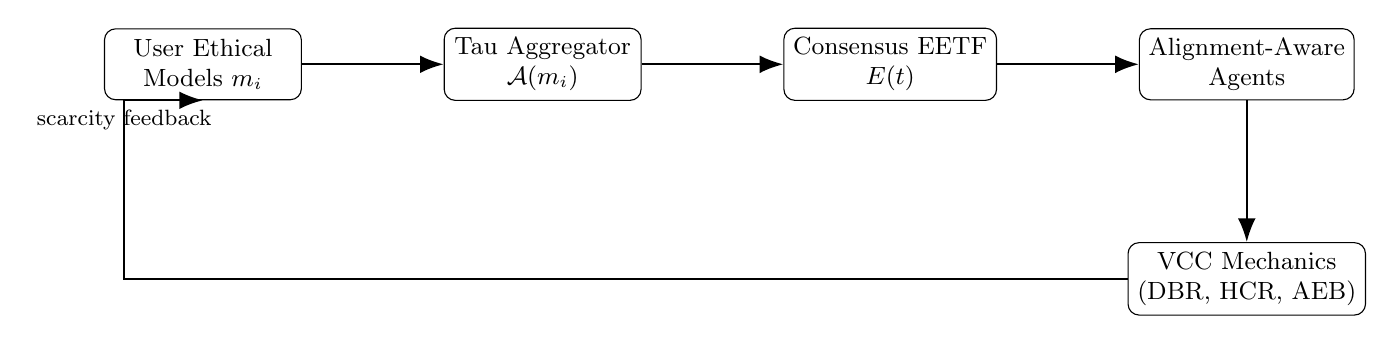
\begin{tikzpicture}[
        node distance=1.8cm,
        every node/.style={font=\small},
        process/.style={rectangle, draw, rounded corners, minimum width=2.5cm, minimum height=0.9cm, align=center},
        arrow/.style={-{Latex[length=3mm]}, thick}
    ]
        \node[process] (models) {User Ethical\\ Models $m_i$};
        \node[process, right=of models] (agg) {Tau Aggregator\\ $\mathcal{A}(m_i)$};
        \node[process, right=of agg] (eetf) {Consensus EETF\\ $E(t)$};
        \node[process, right=of eetf] (agents) {Alignment-Aware\\ Agents};
        \node[process, below=of agents] (vcc) {VCC Mechanics\\ (DBR, HCR, AEB)};
        \draw[arrow] (models) -- (agg);
        \draw[arrow] (agg) -- (eetf);
        \draw[arrow] (eetf) -- (agents);
        \draw[arrow] (agents) -- (vcc);
        \draw[arrow] (vcc.west) -| ([xshift=-1cm]models.south) |- (models.south) node[pos=0.25, below] {\footnotesize scar\-city feedback};
    \end{tikzpicture}
    \caption{Consensus ethics pipeline: user models are aggregated via Tau Language into the EETF signal, which drives alignment-aware agents and VCC mechanisms. Scarcity and burn data feed back into future models.}
    \label{fig:ethics-pipeline}
\end{figure}

\begin{figure}[ht]
    \centering
    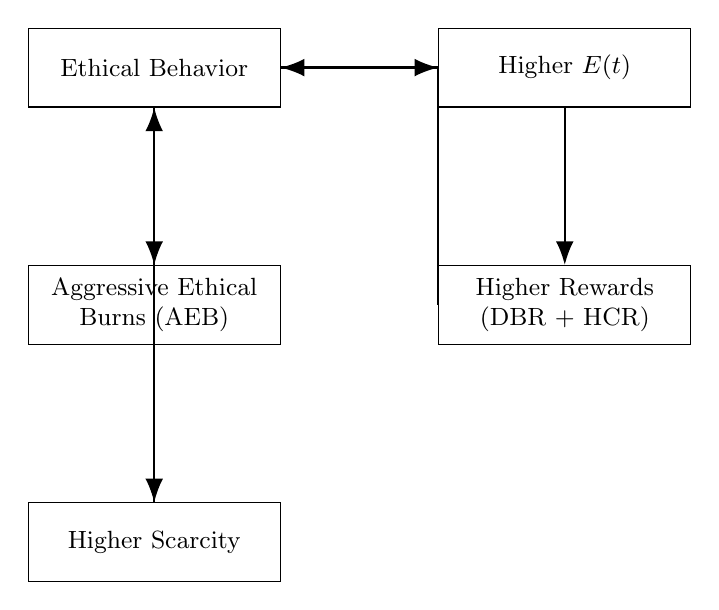
\begin{tikzpicture}[
        node distance=2cm,
        every node/.style={font=\small},
        box/.style={rectangle, draw, minimum width=3.2cm, minimum height=1cm, align=center},
        arrow/.style={-{Latex[length=3mm]}, thick}
    ]
        \node[box] (ethical) {Ethical Behavior};
        \node[box, right=of ethical] (eetf) {Higher $E(t)$};
        \node[box, below=of eetf] (rewards) {Higher Rewards\\ (DBR + HCR)};
        \node[box, below=of ethical] (burns) {Aggressive Ethical\\ Burns (AEB)};
        \node[box, below=of burns] (scarcity) {Higher Scarcity};
        \draw[arrow] (ethical) -- (eetf);
        \draw[arrow] (eetf) -- (rewards);
        \draw[arrow] (rewards.west) |- (ethical);
        \draw[arrow] (ethical) -- (burns);
        \draw[arrow] (burns) -- (scarcity);
        \draw[arrow] (scarcity) -- (ethical);
    \end{tikzpicture}
    \caption{Virtuous Cycle Compounder feedback loops derived from the Alignment Theorem. Ethical behavior increases both rewards and deflationary pressure, reinforcing future ethical choices.}
    \label{fig:vcc-loop}
\end{figure}

\section{Discussion}
\subsection{Ethics as a First-Class Signal}
By letting the community define ``good'' through preference aggregation and logic-based discourse, Tau avoids hard-coded ethics. The Alignment Theorem does not prescribe morality; instead, it ensures that whatever morality the network settles on is economically enforced.

\subsection{Infinite Divisibility vs.\ Supply Limits}
Critiques often note that geometric decays alone do not guarantee non-zero supply. Our framework clarifies this by explicitly modeling the normalized supply in $\mathbb{R}$ while relying on token divisibility (decimal shifting) for practical liveness. This distinction is now embedded both in the Lean assumptions and in the documentation.

\subsection{Future Knowledge Representation}
As Tau adds native knowledge representation and reasoning, agents will be able to query and cite specific ethical models. Broadcasting a user's worldview becomes part of the protocol, enabling richer forms of consensus beyond scalar EETF values (e.g., weighted theories, logic-based disputes, and refutations).

\section{Related Work and Threat Model}
Classical incentive alignment draws on game theory and mechanism design~\cite{vonNeumann,arrow,savage,sen}. Recent blockchain efforts focus on base fee burns (EIP-1559) and MEV mitigation; our proposal differs by letting the community specify ethics declaratively and by coupling burns (AEB) to high EETF as gratitude rather than punishment. The tau-testnet substrate follows the pattern described in~\cite{tautestnet}, where Tau specs are first-class chain data with pointwise revision and extralogical APIs (BLS, commit-reveal, networking).

Threat surfaces include:
\begin{itemize}[leftmargin=*]
    \item \textbf{Aggregator manipulation}: the operator $\mathcal{A}$ must resist Sybil coalitions, spam, and collusion; future work includes formal bounds on adversarial stake/credential weight and diversified aggregation (median, trimmed mean, proof-weighted averages).
    \item \textbf{Pointwise revision safety}: each rule-edit transaction is re-evaluated by the Tau engine, but Lean guards must ensure edits cannot violate constitutional invariants or escalate privileges via extralogical hooks.
    \item \textbf{Oracle / MEV risk}: commit-reveal and oracle monitors (libraries/mev\_oracle\_safety\_v1.tau) need formal verification to guarantee DBR/HCR/AEB do not consume stale or adversarial data.
    \item \textbf{Stress testing}: the simulation suite and tau-testnet traces should cover tail-risk scenarios; `analysis/simulations/run_alignment_simulations.py` and `docs/SIMULATION_RESULTS.md` are first steps.
\end{itemize}
\section{Conclusion}
We have presented an end-to-end ethics-enforcing architecture for Tau Net: ethical knowledge is aggregated via Tau Language, the Alignment Theorem proves that scarcity-driven economics forces rational agents to be ethical, and the Virtuous Cycle Compounder demonstrates the theorem in an educational, verifiable context. This synthesis of knowledge representation, formal proof, and executable specifications offers a template for future decentralized AI alignment research.

\section*{Acknowledgments}
We thank the Tau community for supplying the ethical models, DarkLightX for the VCC visualization work, and the Tau core team for maintaining the interpreter and solver stacks used throughout this research.

\begin{thebibliography}{9}
\bibitem{vccviz}
DarkLightX, ``Virtuous Cycle Compounder Concept Visualizer,'' GitHub repository, 2025. Available at \url{https://github.com/TheDarkLightX/VCC-concept-visualizer}.
\bibitem{tautestnet}
IDNI, ``Tau Testnet Alpha,'' GitHub repository, 2025. Available at \url{https://github.com/IDNI/tau-testnet}.
\bibitem{vonNeumann}
J.~von Neumann and O.~Morgenstern, \emph{Theory of Games and Economic Behavior}, Princeton University Press, 1944.
\bibitem{arrow}
K.~J. Arrow, \emph{Social Choice and Individual Values}, Wiley, 1951.
\bibitem{savage}
L.~J. Savage, \emph{The Foundations of Statistics}, Wiley, 1954.
\bibitem{sen}
A. Sen, \emph{Collective Choice and Social Welfare}, Holden-Day, 1970.
\bibitem{preferencebased}
M. Voorhoeve, ``Can There Be a Preference-Based Utilitarianism?'' in \emph{Oxford Studies in Normative Ethics}, Oxford University Press, 2014.
\bibitem{machineethics}
B. Tomasik, ``Machine Ethics and Preference Utilitarianism,'' Reducing Suffering, 2015. Available at \url{https://reducing-suffering.org/machine-ethics-and-preference-utilitarianism/}.
\bibitem{ca_utilitarian}
T. Everitt and M. Hutter, ``Preference Utilitarianism in Physical World Models,'' arXiv:1504.05603, 2015.
\end{thebibliography}

\end{document}

